\chapter{Conclusions and Outlook}
\label{ch:conclusion}
\graphicspath{{conclusion/fig/}}

In this thesis, we set out to apply energy landscape techniques to study complex macroscale systems, in particular multistable elastic structures. 
However, we found that traditional techniques, such as chain-of-states pathway methods, are often inadequate for these applications.
As a result, we have developed new techniques to study the energy landscapes of these large-scale systems.

In \cref{ch:bitss}, we introduced a new transition state search method, BITSS.
Unlike traditional methods, BITSS does not require any initial estimate for the pathway, making it effective for locating complex pathways without any a priori knowledge of their route.
We have shown that BITSS is compatible with adaptive remeshing techniques, which can offer simultaneous improvements to both efficiency and accuracy.
Furthermore, BITSS has been successfully applied to various challenging energy landscapes, such as where it is locally flat, or even discontinuous.
Therefore, this opens up a range of previously inaccessible problems to energy landscape analysis.

This and several other methods have then been incorporated into an energy landscape software library, `ELLib', as detailed in \cref{ch:software}.
The library is designed to be modular, flexible to use, and may be easily extended to incorporate new methods and potentials.
Additionally, it is designed to utilise parallel methods for calculating potentials, minimisation, and exploring energy landscape for large system sizes.
% However, further work is still required to ensure that some energy landscape methods can fully utilise the scalability offered by parallel computing.


Having developed this new methodology, we then applied it to investigate the behaviour of multistable buckled mesostructures.
We demonstrated in \cref{ch:mesostructures} that our approach can accurately locate stable states and reconfiguration pathways for a range of different structures, with results that match observations from experimentally manipulating the structures.
Moreover, by investigating a table structure we were able to create phase diagrams that highlight how the various states and pathways depend upon the chosen system parameters.
These findings can therefore be used to design a structure with specific functionality for a given application.

In \cref{ch:origami_ribbon} we extended our investigations to explore the effect of origami-inspired creases on the multistability of simple ribbons, which can be used as a building block for many larger structures.
Our results show that the number of creases plays a critical role in the number of available states, with three creases showing the greatest multistability, then quickly reducing to just a single stable state as the number of creases is increased further.
Furthermore, we found that increasing the strain led to changes to the available states and pathways, with a group of states that could be easily interchanged while another was separated by a large barrier.

Taken together, these results provide new insight into how the multistability of buckled mesostructures is affected by various structural and material parameters.
Our methodology and findings outline a process by which these, and other more general structures, may be tailored to obtain chosen states and reconfiguration pathways.
The identified reconfiguration pathways can also be serve as targets for remote actuation, providing a critical step towards developing rapidly reconfigurable devices for applications in soft robotics and deployable structures, among other fields.
This work has thus contributed to advancing the field of multistable elastic structures and has potential implications for a wide range of technological applications.



\section{Future work}
\subsection{Locating multiple pathways}
Many applications have multiple competing pathways between a pair of states.
For example, the snap-through buckling of a clamped beam, \cref{fig:conc-multits}(a), can take one of two asymmetric pathways.
Therefore, we may wish to use a method that enables us to locate these additional pathways.

However, locating multiple pathways between a single pair of minima is a difficult problem that has not been fully addressed by existing methods.
One possibility is to use single-ended TS search methods from the regions around each of the minima, however this is not guaranteed to find all of the TS and those that are found may not be connected to the states of interest.
Another approach is to make initial guesses using a chain-of-states method, but this requires some knowledge of the expected pathways and the initial interpolation may be difficult.
Alternatives are possible, such as transition path sampling \cite{Bolhuis2002} or using molecular dynamics over long time-scales, but these can be very computationally costly.

\begin{figure}[htb]
  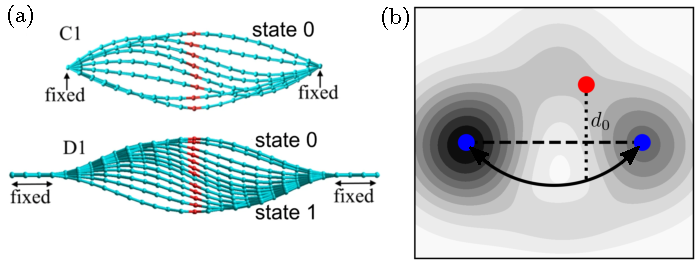
\includegraphics{multits.pdf}
  \caption{
    (a) The asymmetric snap-through buckling pathways for constrained thin sheets (specifically graphene membranes).
    The endpoints are allowed to rotate in the first, and they are fixed in the second.
    An equivalent, reflected pathway is possible in both.
    Adapted with permission from \cite{Yamaletdinov2018}.
    (b) Schematic illustrating a 2D landscape with two pathways, and a possible modified distance metric that would enable BITSS to locate the second TS.
    The pathway's radius of curvature is calculated to set a certain distance $d_0$ from the known TS (red dot).
  }
  \label{fig:conc-multits}
\end{figure}

One possibility would be to extend the BITSS method to locate multiple TS by modifying the distance metric.
Taking inspiration from general relativity, in which mass can curve space-time and reduce the distance between two points, once BITSS has located a TS a ``negative mass'' could be applied, effectively expanding space around that point.
This would result in the two states attempting to move away from the known TS as they converge, and hopefully converging to another.
This could then be repeated to find multiple different transition states that separate the two minima.
Such a method would bear a resemblance to the deflated Newton method\cite{Noack2017}, but for finding multiple TS instead of minima.

Of course attempting to calculate an accurate distance based upon a curved space-time would be exceedingly complicated, however it does provide a useful analogy.
Instead, a simpler approach could be to consider a circular arc between the states that has a radius of curvature that points it away from the TS so that the images would converge a chosen distance away, as illustrated in \cref{fig:conc-multits}(b).
By repeating BITSS and continually increasing this distance bias, it could be possible to locate all available pathways.


\subsection{3D elastic metamaterials}
In this thesis, we have investigated the behavior of two-dimensional elastic structures through the use of a discretised shell model that is particularly effective in analyzing the bending of thin films.
However, this approach is insufficient for studying a variety of complex reconfigurable structures such as three-dimensional mechanical metamaterials, as discussed in \cref{sec:es-metamaterials}.
As a result, a natural extension to our work would be to incorporate a three-dimensional elastic potential, such as one based on the finite element method, to better examine these systems.

Energy landscape analysis could be a promising tool for addressing a wide range of problems associated with mechanical metamaterials.
For example, the effectiveness of collisional energy-absorbing structures\cite{Shan2015,Giri2021} is heavily influenced by material and geometric factors, which modify the energy barriers of the various reconfiguration pathways.
Therefore, by optimising the barriers as we demonstrated in \cref{sec:ell-demo}, we could gain valuable insights into how to maximize the efficiency of these structures.

A similar analysis could be applied to flexible metamaterials that undergo a large-scale, bistable transformation, which are of interest to develop deployable structures \cite{Shang2018,Zareei2020}.
Here, an important consideration is their durability, i.e. how many times they can be reconfigured without breaking, which is found to be inversely correlated with the elastic strain energy during the transition \cite{Shang2018}.
In this case, investigating the minimum energy pathway could provide the structural parameters that minimise the energy barrier, thereby increasing durability, while allowing the structure to remain bistable.

\begin{figure}
  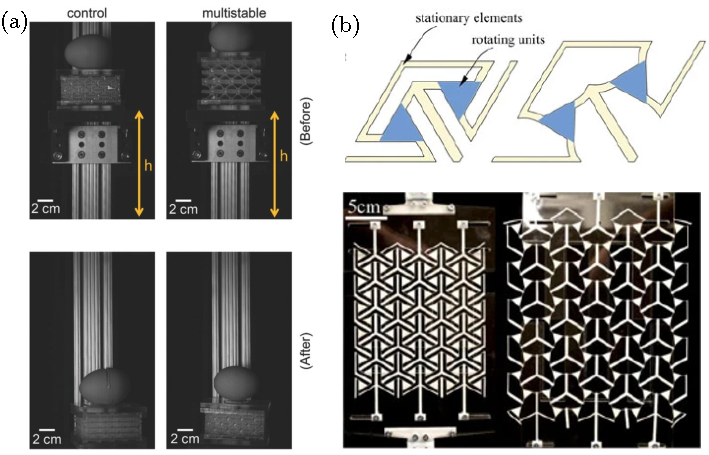
\includegraphics{metamaterials.pdf}
  \caption{
    (a) Energy absorbing structures.
    Adapted with permission from \cite{Shan2015}.
    (b) Bistable auxetic metamaterial that undergoes a transition to a deployed state.
    Adapted with permission from \cite{Shang2018}.
  }
\end{figure}


\subsection{Reconfigurable surface structures for adaptable wetting}
An interesting application of the creased ribbon structures investigated in \cref{ch:origami_ribbon} could be to create an array of adaptable surface structures that could be remotely switched between two states in order to alter the wetting properties of a surface.

For example, it is known that an array of pillars on a surface can keep a droplet in a suspended Cassie--Baxter state where it can exhibit superhydrophobic behaviour.
But this depends upon the geometry of the posts, and if they are further apart the droplet may instead transition to a Wenzel state, sinking into the structure and losing the superhydrophobic behaviour.
These two states could potentially be switched from one to the other using the structure in \cref{fig:conc-wetting}(b), which has one state where the `pillars' are larger with less spacing between then, and another state with smaller pillars and larger spacing.

However, due to their more complicated design, flexible ribbon structures would restricted to larger sizes than a simple pillar geometry, making the Wenzel state more prone to failure.
Energy landscape methods could be used to address this using a similar analysis as performed in \cite{Panter2019a}.
This would provide information as to how the structure should be modified to maximise the energy barrier that prevents the droplet from penetrating the structure.

\begin{figure}
  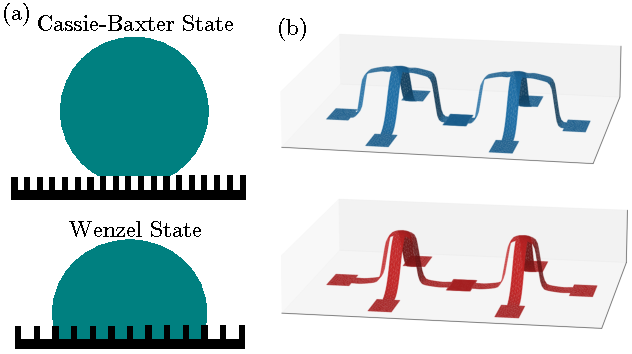
\includegraphics{wetting.pdf}
  \caption{
    (a) Illustration of the Cassie--Baxter and Wenzel states of a droplet on a structured surface.
    (b) An origami-inspired mesostructure with two states that could be used to realise an adaptable wetting surface.
  }
  \label{fig:conc-wetting}
\end{figure}
